\chapter{Visione artificiale}
\label{chap:visione}

\begin{minipage}{12cm}\textit{In questo capitolo verrà trattato il problema della generazione dei set di coppie di punti omologhi usando tecniche di visione. In particolare si utilizzeranno tecniche di Feature Detection e stereoscopia.}
\end{minipage}

\vspace*{1cm}

Nel capitolo \ref{chap:visualObs} si è accennato agli strumenti che sarebbero stati usati al fine della generazione dei suddetti set. In questo capitolo si procederà ad illustrarne il funzionamento con maggior dettaglio e si fornirà una possibile soluzione al problema. Conviene definire per primo il problema che si vuole affrontare.

\begin{prob}
	\label{prob:vis:gensets}
	Sia un osservatore mobile dotato di almeno due fotocamere. Si supponga ancora capace di "catturare", attraverso le suddette fotocamere, coppie di foto in diversi istanti (anche regolari). Allora: 
	\begin{enumerate}
		\item è possibile, utilizzando le informazioni fornite dalle fotocamere, calcolare le coordinate spaziali (in $\mathbb{R}^3$) di un punto del mondo (o più di uno) nel sistema di riferimento solidale all'osservatore?
		\item dato un punto del mondo (o più di uno) per il quale si è riusciti a calcolarne le coordinate spaziali, è possibile individuare lo stesso punto, in un altro istante del tempo, se l'osservatore si è mosso e se lo stesso è ancora visibile?  
	\end{enumerate}
\end{prob}

\section{Feature Detection e Matching}
\label{sec:feature}
Per \textbf{Feature Detection} o \textbf{individuazione dei punti chiave} in italiano, si intende un particolare settore facente parte della branca della visione artificiale, il cui scopo è quello di per l'appunto l'individuazione, la descrizione e il confronto delle Feature. Ma che cosa è una Feature?
In generale risulta difficile fornire una definizione chiara di cosa è una \textbf{Feature} o \textbf{Punto chiave}, può dipendere ad esempio dall'algoritmo che si utilizza o da scelte implementative.


\begin{figure}[h]
	\centering
	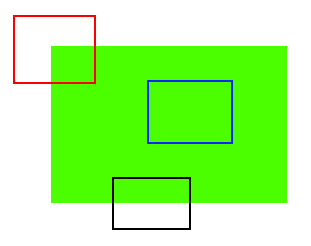
\includegraphics[width=420pt]{imgs/feature_simple.png}
	\caption{Individuazione delle Features.}
	\label{vis:feature:detect}
\end{figure} 

Si faccia ad esempio riferimento alla figura \ref{vis:feature:detect}, si supponga di dover individuare una buon punto chiave, il quale possa essere facilmente riconosciuto e riposizionato. Si consideri per prima la porzione di immagine evidenziata dal riquadro blu; è chiaro che qualora si dovesse scegliere dove posizionare tale blocco, si avrebbero un numero elevatissimo di possibilità ed in nessun caso si potrebbe avere al certezza di un buon posizionamento. Si consideri allora il blocco nero, in questo caso il numero delle possibilità è sicuramente inferiore, infatti esso può essere posizionato solo nel lato inferiore del rettangolo verde in figura. Infine si consideri il blocco rosso, è chiaro che quello in figura è l'unico punto in cui esso può essere posizionato.
L'esempio precedente fornisce un importantissimo spunto ri riflessione su cosa può essere una Feature e cosa no. Infatti sicuramente una porzione di immagine uniforme non può essere un punto chiave; se invece si considerano dei contorni di un oggetto la situazione migliora. In particolare se si considera il contorno di un oggetto e se ne sceglie un punto che abbia una forma o pattern particolare, come ad esempio uno spigolo di un oggetto, risulta molto più facile un eventuale riconoscimento. 

Ovviamente l'esempio precedente risulta estremizzato. Infatti, in un caso reale, le Feature possono essere ruotate e/o scalate e questo complica il problema. Al contempo però, il mondo reale risulta più dettagliato e risulta più difficile avere uno stesso pattern in punti diversi.

Si è fornita, quanto meno in modo informale, una definizione di Feature. Nei prossimi paragrafi con ordine si illustreranno tre algoritmi: il primo adibito all'individuazione delle features, il secondo viene impiegato per la generazione dei descrittori (che come si vedrà sono utilizzati per distinguere i punti chiave in base alle informazioni fornite dall'immagine) ed il terzo è un matcher. 

%\subsection{Definizioni e problema}
%\label{sec:det:def}
\subsection{L'algoritmo FAST}
\label{sec:det:fast}
L'algoritmo FAST (Feature from Accelerated Segment Test) è un algoritmo adibito all'estrazione dei punti chiave da un immagine, sviluppato originariamente da Edward Rosten e Tom Drummond nel 2006 \cite{bib2}. Esistono numerosi algoritmi adibiti a questo scopo, ed alcuni riescono anche ad ottenere risultati più accurati. In accordo con il nome dell'algoritmo però quest'ultimo risulta particolarmente veloce e in generale fornisce risultati molto buoni. In accordo con le specifiche di esecuzione realtime già accennate, pertanto la scelta è ricaduta su quest'ultimo. Inoltre l'algoritmo FAST è privo di licenze a pagamento e può essere liberamente impiegato in progetti sia di ricerca che commerciali. Di seguito se ne illustra il funzionamento.
\newline \newline
Si consideri un pixel $p$, sia $I_p$ la sua intensità e siano fissate una soglia di funzionamento $t$ e un intero $n$. Si vuole verificare se il pixel $p$ può essere considerato una Feature oppure no. 

\begin{figure}[h]
	\centering
	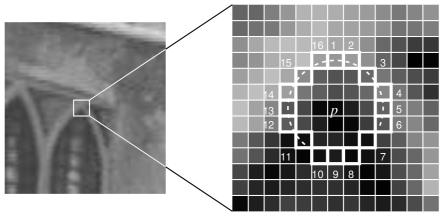
\includegraphics[width=420pt]{imgs/fast_speedtest.jpg}
	\caption{Fast Segment test.}
	\label{vis:feature:Fast}
\end{figure} 
  
 
In accordo con quanto detto nel precedente paragrafo, uno spigolo/angolo può essere considerato una buon punto chiave. Il \textbf{test} ricerca questo tipo di punti e viene effettuato nel modo seguente:
\begin{enumerate}
	\item Si consideri un cerchio di 16 pixel intorno a $p$, evidenziato in figura \ref{vis:feature:detect} dai pixel riquadrati.
	\item Il punto $p$ è uno spigolo se vale che un numero $n$ di pixel appartenenti al suddetto cerchio hanno intensità o tutti maggiore di $I_p + t$ o tutti minore di $I_p - t$.
\end{enumerate}

Osservando sempre la figura \ref{vis:feature:detect} si intuisce la motivazione del test. Infatti uno spigolo, indipendentemente da come è ruotato, avrà una forma convessa. Si intuisce che la buona riuscita del test dipende dalla scelta dei parametri $t, n$, tipicamente si sceglie $n = 12$, $t$ dipende dal tipo di immagini utilizzate.

	Nella pratica si inserisce un \textbf{test veloce} per effettuare una prima scrematura dei punti. Con riferimento alla figura \ref{vis:feature:detect} si controllano solo i pixel 1, 9, 5 e 13. Si verifica se i pixel 1 e 9 hanno una differenza assoluta di intensità rispetto a $p$ maggiore della soglia $t$, in caso si analizzano anche i pixel 5 e 13. Se $p$ è uno spigolo deve valere allora che 3 di tali pixel devono essere più intensi di $p$ e uno meno intenso, dove l'intensità e verificata con al soglia $t$ ovviamente.

Si può notare che se la condizione del test veloce non è verificata allora non c'è modo che il test completo possa avere un buon esito, perché non possono esistere n pixel contigui più intensi o meno intensi di $p$. In generale dei falsi positivi possono superare il test veloce e quindi il testo completo deve essere impiegato per ottenere un risultato corretto.

L'algoritmo allo stato attuale però presenta alcune criticità:
\begin{enumerate}
	\item Per $n < 12$ il test veloce non può essere generalizzato perché un pixel $p$ può superare il test completo anche se solo due dei pixel selezionati sono meno intensi e due più intensi.
	\item L'efficienza del test dipende dalla scelta e dall'ordinamento dei pixel selezionati per il test. In genere però i punti per il successo del test dipende da questi fattori non sono buone feature. 
	\item Molte feature vengono individuate una adiacente all'altra.
\end{enumerate} 

Per risolvere il terzo problema si introduce un ulteriore passo detto \textbf{non-maximal suppression}:
\begin{enumerate}
	\item Si calcola una funzione valore $V$ per tutti i punti chiave individuati. La funzione $V$ per il punto chiave $p$ è pari alla somma della differenza assoluta tra l'intensità di $p$ e i 16 pixel considerati intorno allo stesso durante il test.
	\item Se i punti chiave $p_1$ e $p_2$ sono adiacenti, ovvero hanno una distanza in pixel minore di una soglia $d$, si scarta quello che ha la funzione valore più bassa.
\end{enumerate}
Il precedente test è pensato in modo che, in caso di necessità, vengono scartati i punti chiave meno "marcati" e conseguentemente meno distinguibili. 

L'ultimo passo che può essere impiegato per aumentare le prestazioni del rilevatore FAST è quello di impiegare una \textbf{rete neurale}. Essa può essere addestrata utilizzando i risultati forniti dello stesso FAST durante il funzionamento al fine di sostituire e combinare il test veloce e quello completo. A patto che il set di addestramento sia abbastanza vario e comprensivo di rumore, un addestramento supervisionato può ottenere un buon grado di efficacia ed efficienza. 
% scrivere sta roba%

Si conclude la presentazione dell'algoritmo con alcune riflessioni. FAST è un algoritmo di tipo euristico, come molti altri, ma nel caso generale risulta molto efficace. Per quanto riguarda il test in essere esso ha un basso impatto computazionale, inoltre il test può essere eseguito in parallelo per molti pixel alla volta. Come vedremo esso si presta ad una facile e efficiente implementazione su GPU.

\subsection{L'algoritmo BRIEF}
\label{sec:det:brief}

\subsection{Brute Force matching}
\label{sec:det:bmmatch}


\section{Stereoscopia}
\label{sec:stereo}


%\subsection{Definizioni e problema}
%\label{sec:stereo:def}


\subsection{Modello matematico del sensore fotografico}
\label{sec:stereo:modello}


\subsection{Ricostruzione 3D}
\label{sec:stereo:ric3d}


\section{Soluzione al problema}
\label{sec:vision:solution}


